\chapter{INTRODUÇÃO} \pagenumbering{arabic} % (fold)
\label{cha:introducao}

\section{Motivação} % (fold)
\label{sec:motivacao}

% O que é importante para: nós, comunidade científica, usuários, mercado.

% Apresentar a motivação e justificativa para a realização do trabalho (por exemplo, sua aplicabilidade prática, comparação com alternativas já existentes, potencial de  aprendizado e evolução, etc).

% http://www.uxmatters.com/mt/archives/2009/03/including-recommendations-in-user-interfaces-to-enhance-motivation.phps

 Sistemas de Recomendação sugerem itens que as pessoas possam gostar, baseado em seu comportamento prévio. Fazendo suposições pertinentes sobre o tipo de objetos em que elas estão interessadas, é possível conquistar a sua confiança. A vantagem para os usuários é a facilidade de encontrar a informação, sem ter a árdua tarefa de procurá-la.

 As redes sociais online têm modificado a forma com que as empresas utilizam a comunicação para o comércio. Pessoas estão utilizando a Web para encontrar outras pessoas com interesses similares, fazer compras de forma mais eficiente, aprender sobre produtos e serviços e reclamar sobre produtos malfeitos \cite{marketing_social_web}.

 A Web está rapidamente se tornando a mídia mais importante para o marketing. A tendência é que as pessoas cada vez mais bloqueiem os anúncios indesejados e queiram ter a capacidade de encontrar os produtos relevantes no momento adequado. É nesse contexto que surge a necessidade de uma plataforma que facilite a colaboração e que permita a criação e classificação de conteúdo pelos consumidores, de forma a permitir uma escolha mais inteligente dos melhores produtos e serviços, e ao mesmo tempo criando uma mecanismo de feedback para as empresas interessadas.

 Devido à grande variedade atual de produtos e serviços, as pessoas têm cada vez mais dificuldade nas suas escolhas e na argumentação sobre a possível decisão. Quanto maior for a quantidade de produtos similares de fabricantes diferentes, mais as pessoas se vêem desnorteadas e sem saber se a decisão tomada foi a mais correta.

% paragraph paragraph_name (end)
% section motivação (end)


\section{Objetivos} % (fold)
\label{sec:objetivos}

 O principal objetivo deste projeto é criar um sistema de recomendação baseado em recursos disponíveis na Web, que possibilite a sugestão de itens confiáveis e relevantes ao usuário.

 Este sistema utiliza três algoritmos de recomendação distintos: um baseado em perfis de usuários (RBP), outro baseado em similaridade entre produtos/itens (RBI) e um outro, proposto neste trabalho, que é baseado em uma função de confiança entre usuários (RBC). Este último algoritmo utiliza informações fornecidas pelos próprios usuários, através do uso de uma rede social acoplada ao sistema, para calcular estes índices de confiança.

% section objetivo (end)

\section{Metodologia} % (fold)
\label{sec:metodologia}

 Inicialmente foi realizada uma pesquisa bibliográfica com os assuntos relacionados ao trabalho, como sistemas de recomendação (\textit{recommender systems}), redes sociais (\textit{social networks}), tomada de decisão (\textit{common sense}), Web semântica (\textit{semantic Web}), entre outros. Após isso, esta pesquisa bibliográfica foi detalhada sobre os assuntos que fariam parte do escopo do projeto, como sistemas de recomendação e redes sociais.

 Algumas práticas das metologias de desenvolvimento ágil foram adotadas neste projeto, como o Desenvolvimento Dirigido por Testes (TDD\footnote{Do inglês \textit{Test Driven Development.}}). Nesta prática, sempre que uma nova funcionalidade for adicionada ao sistema, o desenvolvedor deve iniciar o processo testando a mesma. Após executar o teste, em caso de falha o desenvolvedor deve verificar porque o teste falhou e então adicionar o código necessário para corrigi-la. Em uma etapa posterior, o desenvolvedor deve adicionar mais testes para a nova funcionalidade até que ela possa ser considerada pronta.
 
 Outro processo de desenvolvimento de software utilizado no projeto foi a refatoração de código \cite{fowler1999refactoring}. A refatoração de código consiste na mudança da estrutura interna do programa sem afetar o seu comportamento externo. Dessa forma, é possível aprimorar o código fonte existente melhorando a sua legibilidade, aplicando simplificações na estrutura, adequando a paradigmas de programação, melhorando a performance e a extensibilidade.
 
 Foi realizado um experimento prático com a participação de pessoas externas ao projeto para o colhimento de resultados da utilização do sistema proposto.

 Para a formação da base de dados que comporia o cadastro de produtos utilizado no experimento foram escolhidos os seguintes aspectos:

\begin{itemize}
	\item Diversidade de produtos
	\subitem Foram consideradas diversas categorias de produtos para que houvesse uma heterogeneidade no cadastro.
	\item Produtos com alto índice de relevância nas categorias
	\subitem Os produtos mais relevantes em cada categoria foram cadastrados com o intuito da base de dados não ser composta apenas de produtos desconhecidos aos participantes do experimento.
\end{itemize}

 O experimento realizado foi dividido em etapas, sendo que enquanto uma etapa não era concluída por todos os participantes, as etapas subseqüentes não eram iniciadas. Com isso, o desenvolvimento das funcionalidades disponíveis pelo sistema foi gradual, proporcionando a correção de erros nas etapas a serem ainda liberadas.

 Além disso, enquanto o experimento estava no ar, os participantes que já haviam terminado determinada etapa comunicavam espontaneamente por e-mail as dificuldades ou facilidades que tiveram durante a realização da mesma. Isso facilitava a correção imediata de erros com o sistema no ar e a mitigação dos mesmos na etapas seguintes.

 O sistema de recomendação implementado utiliza 3 tipos de algoritmos para realizar as recomendações aos usuários.

\begin{figure}
  \centering
  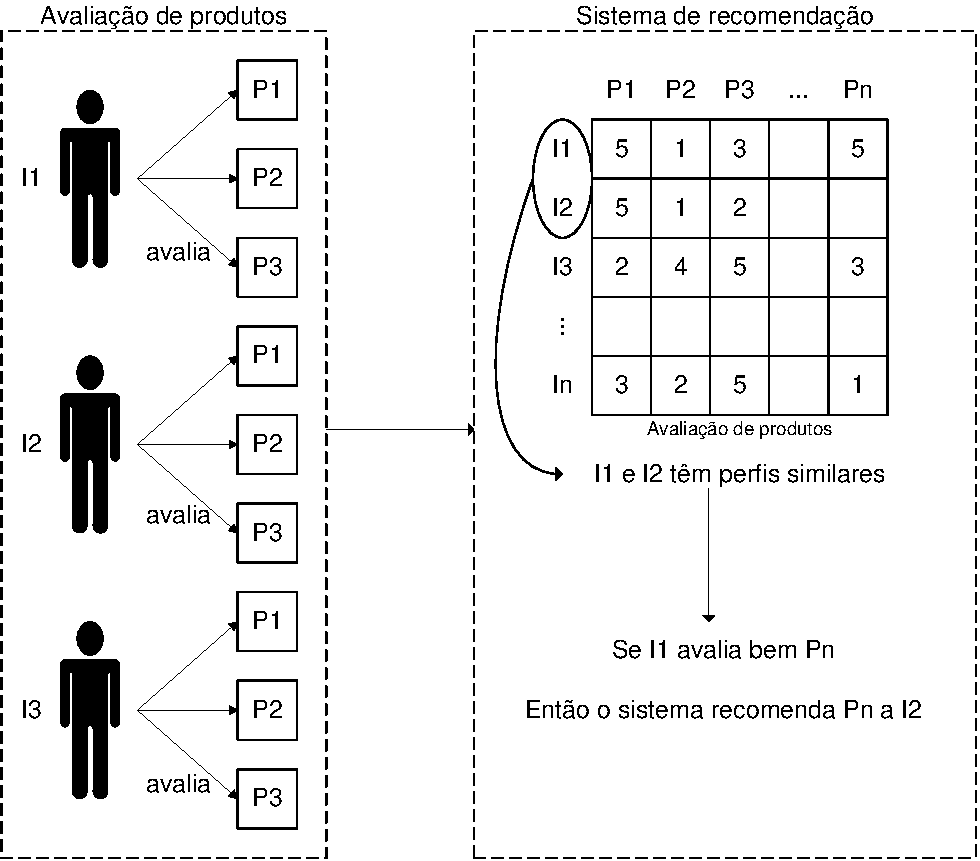
\includegraphics[width=\textwidth]{imagens/RBP}
  \caption{\it RBP: Recomendação com base em similaridade entre perfis}
  \label{fig:RBP}
\end{figure}

 A recomendação com base na similaridade entre perfis de usuários (RBP) utiliza a correlação de Pearson para calcular a semelhança entre os usuários. Como visto na Figura~\ref{fig:RBP} inicialmente os usuários avaliam alguns produtos em comum. Comparando os usuários um-a-um com base nas notas que eles deram aos produtos, calcula-se a correlação de Pearson que resultará em alto grau de similaridade caso os dois usuários tenham avaliado produtos de forma semelhante. Desse modo, se dois usuários têm perfis similares e um deles avalia bem um produto $P{n}$ então o sistema recomenda este produto ao outro usuário.

 A recomendação com base em similaridade entre produtos/itens (RBI) calcula a semelhança entre produtos para realizar as recomendações. Como mostrado na Figura~\ref{fig:RBI} inicialmente os usuários avaliam alguns produtos em comum. O sistema de recomendação utiliza essas informações de avaliação de produtos para calcular uma-a-uma a correlação entre os produtos, calculando a sua distância Euclidiana. Caso dois produtos $P{1}$ e $P{2}$, tenham alto índice de correlação e um usuário avalia bem $P{1}$, então o sistema também recomenda $P{2}$ a ele.

\begin{figure}
  \centering
  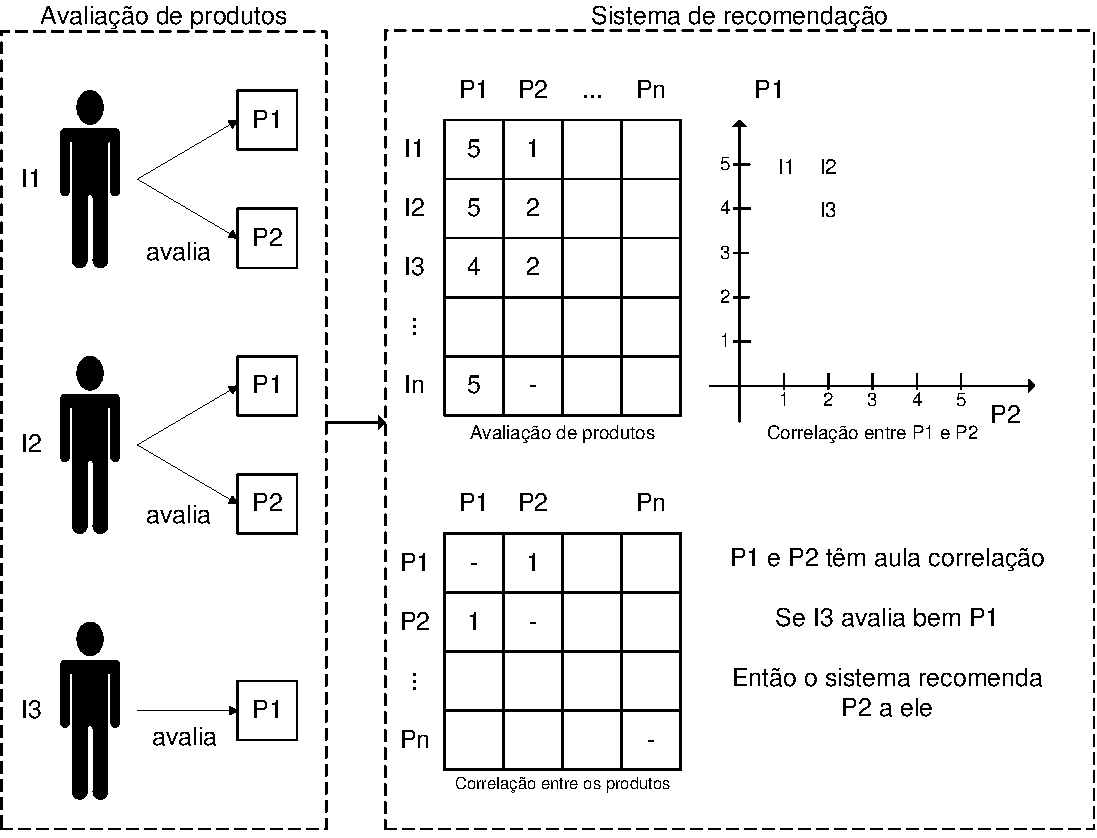
\includegraphics[width=\textwidth]{imagens/RBI}
  \caption{\it RBI: Recomendação com base em similaridade entre produtos}
  \label{fig:RBI}
\end{figure}

 Os dois algoritmos introduzidos anteriormente são conhecidos na comunidade científica e muito utilizados entre os sistemas de recomendação atuais. O algoritmo proposto pelo grupo é a recomendação com base em confiança (RBC). Neste caso, inicialmente um usuário avalia alguns produtos e depois recomenda um deles a outras pessoas. Depois dessas pessoas terem avaliado o produto recomendado, o sistema de recomendação calcula o índice de confiança entre o usuário recomendador e o usuário que recebeu a recomendação. Quanto melhor o produto recomendado for avaliado, maior será o índice de confiança que este usuário tem naquele que fez a recomendação. Caso o índice de confiança seja alto, o sistema recomenda produtos bem avaliados pelo usuário recomendador ao usuário recomendado. O RBC é ilustrado na Figura~\ref{fig:RBC}.

\begin{figure}
  \centering
  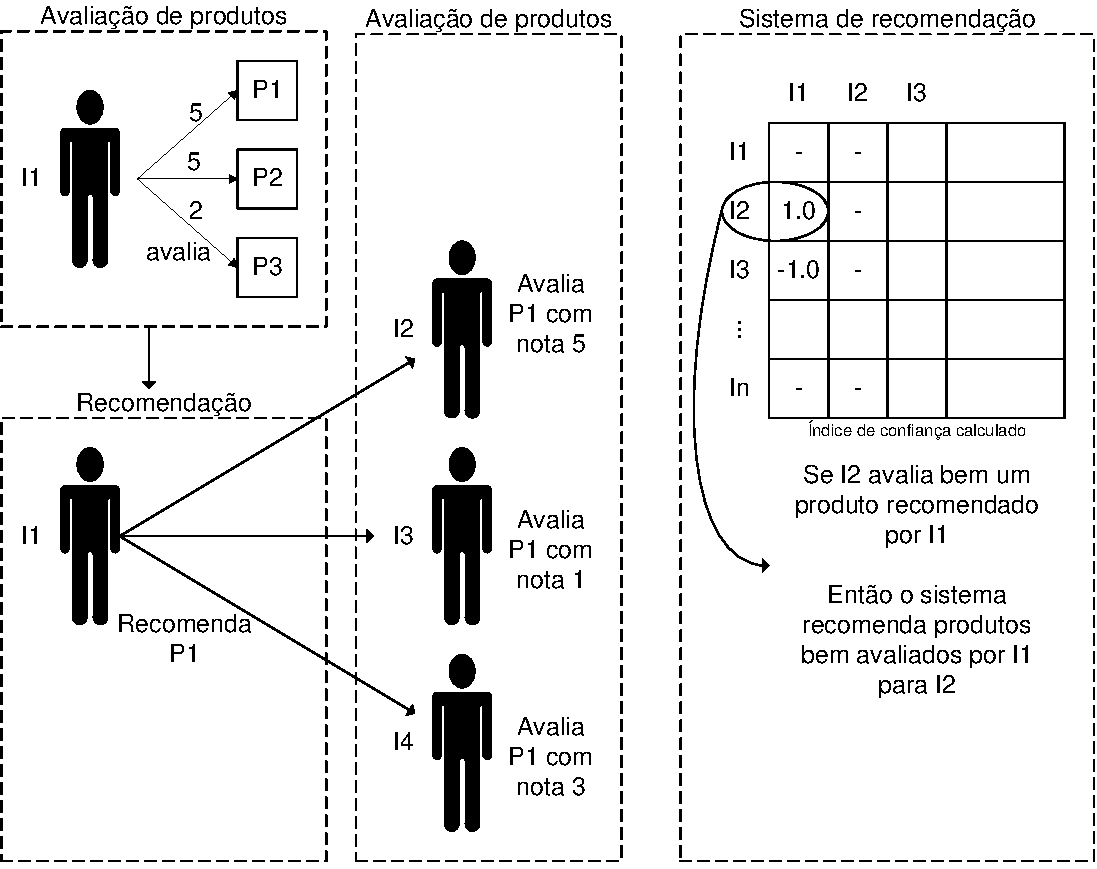
\includegraphics[width=\textwidth]{imagens/RBC}
  \caption{\it RBC: Recomendação com base em confiança}
  \label{fig:RBC}
\end{figure}

 Após o desenvolvimento e implementação dos algoritmos, o sistema foi testado por uma coleção de 60 pessoas, agrupadas em 12 classes, sendo que cada classe indica um grupo de amigos, isto é, pessoas que confiam umas nas outras. Os resultados dos diferentes algoritmos de recomendação foram então comparados através de testes estatísticos.

 O controle de versão do código fonte criado foi feito com o SVN\footnote{Do inglês \textit{Subversion}. SVN é um sistema de controle de versão de documentos quaisquer.}. Esse sistema de controle ajudou muito no desenvolvimento paralelo do sistema do projeto por todos os integrantes do grupo. Os arquivos utilizados durante todo o desenvolvimento do projeto também foram versionados com o SVN.

% section metodologia (end)

\section{Organização} % (fold)
%\label{sec:organização}

 Este trabalho está estruturado em 6 capítulos e 3 apêndices.
 
 O capítulo 1 consiste nesta introdução onde são apresentados a motivação da realização deste projeto, os objetivos a serem alcançados com o trabalho e a metodologia utilizada no projeto.
 Já o capítulo 2 descreve os conceitos básicos empregados e utilizados durante a realização do projeto.
 No capítulo 3,	especifica-se o projeto mostrando a sua visão geral, descrição, funcionalidades e os detalhes técnicos da sua implementação.
 O capítulo 4 apresenta a especificação do experimento realizado durante o projeto para colhimento de dados.
 No capítulo 5 são mostradas as análises e os resultados obtidos do sistema com a realização do experimento.
 O capítulo 6 contém as considerações finais deste trabalho, sendo composto da conclusão e das propostas de trabalhos futuros.
 
 No apêndice A são mostrados os resultados dos testes de hipótese realizados sobre a amostra obtida com o experimento.
 O apêndice B contém o Termo de Consentimento Livre e Esclarecido (TCLE) utilizado no experimento.
 Já o apêndice C descreve as instruções apresentadas aos participantes do experimento para a realização das tarefas de cada etapa.

% section organização (end)

% chapter web_social (end)